\documentclass[tikz,border=15pt]{standalone}
\usetikzlibrary{decorations.pathreplacing, arrows.meta}
\begin{document}
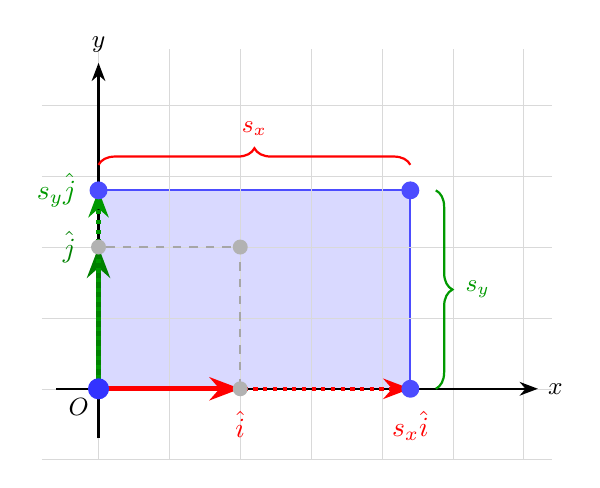
\begin{tikzpicture}[>=Stealth, scale=1.8]

    \def\sx{2.2}
    \def\sy{1.4}
    \def\orig{1.0}

    % ── Scaled square FIRST (behind everything) ───────────────────────────────
    \filldraw[fill=blue!15, draw=blue!70, thick]
        (0,0) rectangle ({\sx*\orig}, {\sy*\orig});

    % ── Grid ─────────────────────────────────────────────────────────────────
    \draw[help lines, step=0.5, gray!30] (-0.4,-0.5) grid (3.2,2.4);

    % ── Axes ─────────────────────────────────────────────────────────────────
    \draw[->, thick] (-0.3, 0) -- (3.1, 0) node[right, font=\small] {$x$};
    \draw[->, thick] (0, -0.35) -- (0, 2.3) node[above, font=\small] {$y$};

    % Origin
    \node[below left, font=\small] at (0,0) {$O$};

    % ── Original square: dashed ───────────────────────────────────────────────
    \draw[dashed, thick, gray!70] (0,0) rectangle (\orig,\orig);

    % ── Original unit vectors — red î, green ĵ ────────────────────────────────
    \draw[->, very thick, red, line width=1.8pt] (0,0) -- (1,0)
        node[below=4pt, font=\normalsize] {$\hat{i}$};
    \draw[->, very thick, green!50!black, line width=1.8pt] (0,0) -- (0,1)
        node[left=4pt, font=\normalsize] {$\hat{j}$};

    % ── Scaled unit vectors — dotted ──────────────────────────────────────────
    \draw[->, red, very thick, line width=1.5pt, dotted] (0,0) -- ({\sx}, 0)
        node[below=4pt, font=\normalsize, red] {$s_x\hat{i}$};
    \draw[->, green!60!black, very thick, line width=1.5pt, dotted] (0,0) -- (0, {\sy})
        node[left=4pt, font=\normalsize, green!60!black] {$s_y\hat{j}$};

    % ── Corner dots ───────────────────────────────────────────────────────────
    \foreach \x/\y in {{\sx*\orig}/0, {\sx*\orig}/{\sy*\orig}, 0/{\sy*\orig}}
        \fill[blue!70] (\x,\y) circle (1.8pt);
    \foreach \x/\y in {\orig/0, \orig/\orig, 0/\orig}
        \fill[gray!60] (\x,\y) circle (1.5pt);

    % ── Origin dot ────────────────────────────────────────────────────────────
    \filldraw[blue!80] (0,0) circle (2pt);

    % ════════════════════════════════════════════════════════════════════════
    % CURLY BRACES
    % ════════════════════════════════════════════════════════════════════════

    % RED — s_x: brace ABOVE the scaled rectangle top edge
    \draw[decorate, decoration={brace, amplitude=6pt},
          thick, red]
        (0, {\sy*\orig+0.18}) -- ({\sx*\orig}, {\sy*\orig+0.18})
        node[midway, above=7pt, font=\small, red] {$s_x$};

    % GREEN — s_y: brace on RIGHT side of scaled rectangle
    \draw[decorate, decoration={brace, amplitude=6pt, mirror},
          thick, green!60!black]
        ({\sx*\orig+0.18}, 0) -- ({\sx*\orig+0.18}, {\sy*\orig})
        node[midway, right=7pt, font=\small, green!60!black] {$s_y$};

\end{tikzpicture}
\end{document}